% Manuscript. Build: pdflatex and bibtex as in ../README.md. Every number in the text comes from numbers.tex
% and the tab_*.tex fragments, which ../code/make_numbers.py writes from the frozen search results in ../data/
% (in the development repository, engine/data/swarm_cache).
\documentclass[11pt]{article}
\usepackage[letterpaper,margin=1in]{geometry}
\usepackage[T1]{fontenc}
\usepackage{lmodern}
\usepackage{amsmath,amssymb,amsthm}
\usepackage{array}
\usepackage{booktabs}
\usepackage{microtype}
\usepackage[font=small,skip=4pt]{caption}
\usepackage{url}
\usepackage{etoolbox}
\apptocmd{\thebibliography}{\raggedright}{}{}
\usepackage{pgfplots}
\pgfplotsset{compat=1.18}
\usepackage[hidelinks]{hyperref}

\hypersetup{
  pdftitle={Excluding Classical Cipher Families for the 1939 D'Agapeyeff Challenge: Key-Free Counts and Searches with Demonstrated Power},
  pdfauthor={Chase Hendrick}}

\newtheorem{proposition}{Proposition}
\theoremstyle{definition}
\newtheorem{remark}{Remark}

% Written by ../code/make_numbers.py from the frozen search results. Do not edit by hand.
% dagapeyeff-corpus.json sha256 8c1ad2ca5f44057a23451ef61ffece5d204eaa12b39072a166e78fed6e8c8a7c
% dagapeyeff-columnar.json sha256 583966c2f0cfffa1fa01490b270109e6e70bfe4ce22661e9806cbc18463de6d9
% dagapeyeff-columnar14c.json sha256 adcb8dfda37b119996710b187b1b1477879d0f9de81dbdac5701c1272995b43a
% dagapeyeff-exhaustive.json sha256 85b5bfd3d6d71e1fa64d899c6c214bed216f738b29823aa6398bef3d88c5c2f2
% dagapeyeff-exhaustive10.json sha256 d1097484efb7d9f7dc808251f41171f01c4dddca904ee87fe5c1068f424544a4
% dagapeyeff-double.json sha256 7f8d191d903dd50e4ab4e6c0d346224072a4d72d8658bc8f0ee8efe60a73da00
% dagapeyeff-keywords.json sha256 18f140920246793d1fc3d68a0bddc3661ab393d6e59b229e77d95ad5b3923f90
% dagapeyeff-foursquare.json sha256 c0363a62546471860a3cc7ca5f1d36c0c0063feaac3d0a889cc58302e96fe665
% dagapeyeff-pairmap.json sha256 b8b84f1cbfc620b8582437bb9c45f13f6ac56205b3ef4f9f733a1835cab3afe7
% dagapeyeff-grillec.json sha256 a60214133d781a14a3911d2dcdf5796e7174e94431258bd0e5289c17041fc268
% dagapeyeff-quick.json sha256 c728c0a82b44b7032f947f1428976fd5a520f373dd54b3fc41edb706bfdd1bd9
% dagapeyeff-homophone.json sha256 5dd228d32081e205bae102e673a8894df74046c6c70bd4ad6b39e59de51e4c20
% dagapeyeff-additive.json sha256 a4c5cc86561c91a245fb7ea9f92e2a6a1fffdf0b25986982fb2d395fb2b68755
% dagapeyeff-direction.json sha256 1a792ccac818b87afcb54b85d1b46c7f75020ecfcc1e320b0a7ab20f0aa22084
% dagapeyeff-errors.json sha256 c320fb539fae677d020c0bf3e277b14b5e9dfe42a2ecfc9455e4ebf7544d2c95
% dagapeyeff-italian.json sha256 9fccff429a9e27f25ebea4881dab9406e351d04b40878970870153face6621c0
% dagapeyeff-screen.json sha256 62bd263ce0b9471de032562d6384930142478138be4d80e02bfffe0be4dd722b
% dagapeyeff-latin.json sha256 87ff95c1141bd3683c634e3e66d9edae3dbe8705081de6e42357cb28987fbfb5
% dagapeyeff-fskeyed.json sha256 6b4ec1b72895836b4e285fa0cb32551561d51986d05c58ed0621637bc0b85709
% dagapeyeff-latin14.json sha256 088888da6a4119add3e684e5fad0a2ac8d8b2555ca4a72619c1e199ab935e32c
% dagapeyeff-tongues.json sha256 acc91ddd75d23c43844e0d24c568964d6df66107b863bb106939e15c9104a8a7
% dagapeyeff-romanian-wide.json sha256 2694b1303e23162756f153cb8cf20579484acf1a6a418aedd5f08a378177a38a
% dagapeyeff-keyedsquares.json sha256 ffc03811a08c441f0a9ec956c3bd099c23fab54767de84d5cd1cff8e1e46db84
% dagapeyeff-nomessage.json sha256 86a68123ba4ee443ff332bbfee54daeaa71ea20ad2606b460f20f89227c78830
% dagapeyeff-latinmore.json sha256 6ec5a4c3eac5a9b1d9af2b7ac3d9231cb3209e0c37ef1421baeed4a32238b8ee
% dagapeyeff-latinshift.json sha256 2e145ddf575030e2d1f88d6ebc5e326c647e867ad7f204b611ac615e45828b33
% dagapeyeff-alllanguages.json sha256 7cfae933a6193855bc173a684c73526a55c2d68f04202b2016fcf520791d2a27
% dagapeyeff-russian.json sha256 078d368d80972a143ee2bc6e0ab9e76a1ac834f60a2bf7d36de40df5726a7c2c
% dagapeyeff-esperanto.json sha256 e8a08c70f4118c4b26ed9edfccba248c6e646b5d132043999d091e0fb53aa014
% dagapeyeff-latinlib.json sha256 1df03e9388d227e1eb9cc30ec8a7562416686ab0066c2825d9eacdf8b0709e66
% dagapeyeff-latinlibrary.json sha256 a5125e5cdf46777f46e13971bfe0f275081a3ffcf35a321421d7b34757e08842
% dagapeyeff-latinw.json sha256 bb4802299aadd20fb53d0a7d18b73ffda3b8030d83827f94d54661d43e14301e
% dagapeyeff-shiftgap.json sha256 797856a17f1d5956103f243938b6c1d6d66615f2bd68af437e6bef88d3959120
% dagapeyeff-reseed.json sha256 92ec3d646cbd09da4f19a2ea00bfb28d929d6c0b1ad0a513daff47b1b2f2b677
% dagapeyeff-latinsmall.json sha256 d4889f28a06d74ed47bbf27f558177302c012bef9ae4475cd52e380bc6a05835
% dagapeyeff-rarecolumn.json sha256 13709d7547ceb027d3a9fa6b84f7e30b47565e74ec9a85122db47afec3319958
% dagapeyeff-latinwords.json sha256 d11a102cc5439f1520a66975deba5905759b27ec615d602f637ac3b7af85858d
% dagapeyeff-latingrille.json sha256 b186590adc9008ffe759934f959f2e0d8a3501460a2fc004800dcd130e147ce2
% dagapeyeff-latindouble.json sha256 a2ada4f8ec8fa43c2a8844efb6cf1503a98e0e2451a1d5afcaba91b1eedc9b34
\newcommand{\addAsHighMin}{0}
\newcommand{\addBest}{\ensuremath{-3.3261}}
\newcommand{\addCases}{24}
\newcommand{\addDraws}{16{,}470}
\newcommand{\addFewest}{20}
\newcommand{\addPlanted}{12}
\newcommand{\addPlantedLow}{\ensuremath{-2.0789}}
\newcommand{\addReaching}{0}
\newcommand{\addRecovered}{11}
\newcommand{\addRestarts}{4}
\newcommand{\addShuffles}{3}
\newcommand{\addSteps}{4{,}000{,}000}
\newcommand{\addTopRows}{177}
\newcommand{\addTopRowsEnglish}{178}
\newcommand{\allBigRateHigh}{112}
\newcommand{\allEstonianFewest}{4}
\newcommand{\allEstonianMedian}{\ensuremath{28}}
\newcommand{\allLanguages}{98}
\newcommand{\allLatinMedian}{\ensuremath{22}}
\newcommand{\allLatinRate}{1{,}201}
\newcommand{\allListed}{134}
\newcommand{\allOthersMedianLow}{\ensuremath{25}}
\newcommand{\allSecondRate}{394}
\newcommand{\allSecondRateLetters}{58{,}624}
\newcommand{\allSecondRateName}{Buryat}
\newcommand{\allSkippedEmpty}{12}
\newcommand{\allSkippedScript}{22}
\newcommand{\allSkippedShort}{2}
\newcommand{\allSkippedShortMost}{16{,}354}
\newcommand{\caCells}{\ensuremath{-3.4667}}
\newcommand{\caCellsHigh}{7}
\newcommand{\cellsChi}{\ensuremath{34.23}}
\newcommand{\cellsDistinct}{18}
\newcommand{\cellsLargest}{20}
\newcommand{\coincidenceA}{\ensuremath{0.0423}}
\newcommand{\coincidenceB}{\ensuremath{0.0369}}
\newcommand{\coincidenceEnglishLow}{\ensuremath{0.0503}}
\newcommand{\coincidenceShuffles}{2{,}000}
\newcommand{\coincidenceShufflesA}{519}
\newcommand{\coincidenceShufflesB}{1{,}910}
\newcommand{\coincidenceWindows}{373}
\newcommand{\corpusAllThree}{0}
\newcommand{\corpusClosestDistance}{8}
\newcommand{\corpusLetters}{1{,}916{,}398}
\newcommand{\corpusMedianErrors}{28}
\newcommand{\corpusWindows}{479{,}051}
\newcommand{\dirAsHigh}{7}
\newcommand{\dirBest}{\ensuremath{-3.2848}}
\newcommand{\dirPlanted}{4}
\newcommand{\dirPlantedLow}{\ensuremath{-2.0333}}
\newcommand{\dirRecovered}{4}
\newcommand{\dirShuffleBestHigh}{\ensuremath{-2.9593}}
\newcommand{\dirShuffleBestLow}{\ensuremath{-3.3338}}
\newcommand{\dirShuffles}{8}
\newcommand{\dirTopScore}{\ensuremath{-3.7735}}
\newcommand{\dirTopTransform}{delay 115}
\newcommand{\dirTopZ}{\ensuremath{3.41}}
\newcommand{\dirTransforms}{363}
\newcommand{\doubleBelow}{50}
\newcommand{\doubleCases}{50}
\newcommand{\eoFewest}{9}
\newcommand{\eoLetters}{948{,}257}
\newcommand{\eoMedian}{\ensuremath{28}}
\newcommand{\errBestFewest}{15}
\newcommand{\errBestMedian}{\ensuremath{29}}
\newcommand{\errCells}{\ensuremath{-3.9003}}
\newcommand{\errEightLow}{\ensuremath{-2.4865}}
\newcommand{\errEightRight}{95}
\newcommand{\errLevel}{48}
\newcommand{\errLevelRight}{24}
\newcommand{\errRandomDraws}{286{,}496}
\newcommand{\errRandomFewest}{13}
\newcommand{\errSixteenLow}{\ensuremath{-3.0820}}
\newcommand{\errWindows}{5{,}116}
\newcommand{\exAboveAll}{10}
\newcommand{\exAboveChance}{6}
\newcommand{\exAboveP}{\ensuremath{0.055}}
\newcommand{\exCasesAll}{24}
\newcommand{\exhaustiveCases}{24}
\newcommand{\exhaustiveCellsLargest}{\ensuremath{0.0698}}
\newcommand{\exhaustivePlantedSmallest}{\ensuremath{0.0345}}
\newcommand{\exhaustiveRegroupedLargest}{\ensuremath{0.0447}}
\newcommand{\fsCellsBest}{\ensuremath{-3.5543}}
\newcommand{\fsCellsHigh}{18}
\newcommand{\fsCellsLow}{13}
\newcommand{\fsKeyedDraws}{7{,}400}
\newcommand{\fsKeyedFewest}{20}
\newcommand{\fsKeyedReaching}{0}
\newcommand{\fsPlanted}{6}
\newcommand{\fsPlantedLow}{\ensuremath{-2.0150}}
\newcommand{\fsRecovered}{4}
\newcommand{\fsRegroupedA}{21}
\newcommand{\fsRegroupedB}{19}
\newcommand{\fsRegroupedBest}{\ensuremath{-3.3427}}
\newcommand{\fsRestarts}{10}
\newcommand{\fsShuffles}{20}
\newcommand{\fsShufflesMin}{9}
\newcommand{\fsStandardFewest}{21}
\newcommand{\fsStandardWindows}{370}
\newcommand{\fsSteps}{1{,}000{,}000}
\newcommand{\fskReaching}{15}
\newcommand{\fskWindows}{15}
\newcommand{\gapCatalan}{\ensuremath{1.14}}
\newcommand{\gapEnglishLow}{\ensuremath{1.14}}
\newcommand{\gapHom}{\ensuremath{0.89}}
\newcommand{\gapHomTab}{\ensuremath{0.88}}
\newcommand{\gapLatin}{\ensuremath{0.68}}
\newcommand{\gapLatinHigh}{\ensuremath{1.86}}
\newcommand{\gapLatinLow}{\ensuremath{0.45}}
\newcommand{\gapLatinRows}{6}
\newcommand{\gapLatinUnder}{5}
\newcommand{\gapLatinUnderHigh}{\ensuremath{0.97}}
\newcommand{\gapRomanian}{\ensuremath{0.48}}
\newcommand{\gapRomanianTab}{\ensuremath{0.48}}
\newcommand{\gapRows}{18}
\newcommand{\gapUnderOne}{7}
\newcommand{\grilleJoint}{0 of 4}
\newcommand{\grilleJointHolesHigh}{18}
\newcommand{\grilleJointSteps}{8{,}000{,}000}
\newcommand{\grilleKnown}{4 of 4}
\newcommand{\grilleSeeded}{0 of 4}
\newcommand{\heldAusten}{12{,}799}
\newcommand{\heldDoyle}{7{,}592}
\newcommand{\heldWells}{16{,}000}
\newcommand{\homCap}{36}
\newcommand{\homCells}{\ensuremath{-3.1312}}
\newcommand{\homCellsAsHigh}{6}
\newcommand{\homPlanted}{6}
\newcommand{\homPlantedLow}{\ensuremath{-1.9796}}
\newcommand{\homRecovered}{6}
\newcommand{\homRegrouped}{\ensuremath{-2.8590}}
\newcommand{\homRegroupedAsHigh}{3}
\newcommand{\homShuffles}{8}
\newcommand{\itAsHigh}{5}
\newcommand{\itCells}{\ensuremath{-4.5563}}
\newcommand{\itErrRecovered}{4}
\newcommand{\itFewest}{9}
\newcommand{\itLetters}{1{,}026{,}120}
\newcommand{\itMedian}{\ensuremath{28}}
\newcommand{\itRecovered}{4}
\newcommand{\itWindows}{256{,}482}
\newcommand{\keywordCells}{\ensuremath{0.8161}}
\newcommand{\keywordCount}{379{,}521}
\newcommand{\keywordNullHigh}{\ensuremath{0.8290}}
\newcommand{\keywordOrders}{2{,}208{,}702}
\newcommand{\keywordPlants}{6}
\newcommand{\keywordPlantsFirst}{4}
\newcommand{\keywordPlantsLow}{\ensuremath{0.9661}}
\newcommand{\ksPlanted}{6}
\newcommand{\ksRecovered}{0}
\newcommand{\ksSteps}{40{,}000{,}000}
\newcommand{\ksWrong}{\ensuremath{-2.5078}}
\newcommand{\laBest}{\ensuremath{-3.9424}}
\newcommand{\laBestAsHigh}{7}
\newcommand{\laClassicalLow}{\ensuremath{-3.3036}}
\newcommand{\laErrRecovered}{6}
\newcommand{\laFourteenDone}{\ensuremath{-4.0104}}
\newcommand{\laFourteenDoneHigh}{6}
\newcommand{\laFourteenPlanted}{8}
\newcommand{\laFourteenRecovered}{8}
\newcommand{\laFourteenRegroupedHigh}{1}
\newcommand{\laFourteenShuffles}{10}
\newcommand{\laFourteenUndone}{\ensuremath{-3.7074}}
\newcommand{\laFourteenUndoneHigh}{8}
\newcommand{\laRecovered}{6}
\newcommand{\laSquare}{\ensuremath{-4.5513}}
\newcommand{\laSquareAsHigh}{5}
\newcommand{\laTrainLetters}{1{,}983{,}658}
\newcommand{\latinLettersAll}{\ensuremath{59.8}}
\newcommand{\latinWithinTwo}{0}
\newcommand{\ldLarge}{0}
\newcommand{\ldSix}{1}
\newcommand{\ldSixOf}{3}
\newcommand{\ldSmall}{6}
\newcommand{\ldSmallOf}{6}
\newcommand{\lgExact}{4}
\newcommand{\lgLow}{0}
\newcommand{\lgLowHigh}{69}
\newcommand{\lgLowLow}{65}
\newcommand{\lgMid}{1}
\newcommand{\lgMidHigh}{82}
\newcommand{\lgMidLow}{77}
\newcommand{\lgNested}{0}
\newcommand{\lgNestedHoles}{19}
\newcommand{\lgNestedOf}{8}
\newcommand{\lgPlanted}{4}
\newcommand{\libFewest}{4}
\newcommand{\libLetters}{8{,}944{,}241}
\newcommand{\libSources}{21}
\newcommand{\llFewest}{3}
\newcommand{\llLetters}{50{,}826{,}522}
\newcommand{\llPages}{1{,}516}
\newcommand{\llWithinFour}{91}
\newcommand{\lmFsCellsHigh}{7}
\newcommand{\lmFsRecovered}{3}
\newcommand{\lmHomRecovered}{2}
\newcommand{\lmShiftDraws}{9{,}774}
\newcommand{\lmShiftFewest}{16}
\newcommand{\lmShiftReaching}{1}
\newcommand{\lsAbove}{5}
\newcommand{\lsBest}{\ensuremath{-3.9855}}
\newcommand{\lsCases}{36}
\newcommand{\lsPlanted}{18}
\newcommand{\lsRecovered}{15}
\newcommand{\lsmAbove}{4}
\newcommand{\lsmBest}{\ensuremath{-3.93}}
\newcommand{\lsmCases}{32}
\newcommand{\lsmPlanted}{48}
\newcommand{\lsmRecovered}{48}
\newcommand{\lsmWeakestFound}{\ensuremath{-2.96}}
\newcommand{\lwAsHighLow}{1}
\newcommand{\lwCellsHigh}{\ensuremath{-3.57}}
\newcommand{\lwCellsLow}{\ensuremath{-4.21}}
\newcommand{\lwPlanted}{40}
\newcommand{\lwRecovered}{39}
\newcommand{\lwWeakestFound}{\ensuremath{-2.95}}
\newcommand{\lwdAbove}{59}
\newcommand{\lwdCellsAsHigh}{3}
\newcommand{\lwdCellsBest}{13}
\newcommand{\lwdCleanHigh}{84}
\newcommand{\lwdCleanLow}{42}
\newcommand{\lwdErrMax}{32}
\newcommand{\lwdPlanted}{60}
\newcommand{\lwdRegroupedAsHigh}{3}
\newcommand{\lwdRegroupedBest}{10}
\newcommand{\lwdSearches}{41}
\newcommand{\lwdShuffles}{4}
\newcommand{\lwdVocab}{19{,}400}
\newcommand{\lwdWorstHigh}{31}
\newcommand{\lwdWorstLow}{17}
\newcommand{\lwdWorstPlanted}{12}
\newcommand{\lwdWorstRecovered}{11}
\newcommand{\nmCellNull}{20{,}000}
\newcommand{\nmDone}{19}
\newcommand{\nmFamilyP}{\ensuremath{0.2814}}
\newcommand{\nmFixed}{8}
\newcommand{\nmGrille}{3}
\newcommand{\nmPlantNull}{2{,}000}
\newcommand{\nmPlanted}{20}
\newcommand{\nmRandom}{1}
\newcommand{\nmShift}{10}
\newcommand{\nmSmallestP}{\ensuremath{0.0138}}
\newcommand{\nmSquare}{19}
\newcommand{\nmStatistics}{30}
\newcommand{\nmUndone}{2}
\newcommand{\pairCellsA}{79}
\newcommand{\pairCellsAMany}{29{,}336}
\newcommand{\pairCellsB}{80}
\newcommand{\pairCellsBMany}{11{,}539}
\newcommand{\pairRegrouped}{85}
\newcommand{\pairRegroupedAMany}{325}
\newcommand{\pairRegroupedBMany}{161}
\newcommand{\quickBest}{\ensuremath{-3.2848}}
\newcommand{\quickPlanted}{6}
\newcommand{\quickPlantedLow}{\ensuremath{-2.1362}}
\newcommand{\quickRecovered}{6}
\newcommand{\quickShuffleBestAsHigh}{0}
\newcommand{\quickShuffleBestHigh}{\ensuremath{-3.3085}}
\newcommand{\quickShuffleBestLow}{\ensuremath{-3.4798}}
\newcommand{\quickShuffles}{8}
\newcommand{\quickVariants}{28}
\newcommand{\rcCellsRest}{188}
\newcommand{\rcClassicalFewest}{16}
\newcommand{\rcEnglishFewest}{19}
\newcommand{\rcLatinFewest}{14}
\newcommand{\rcPacked}{0}
\newcommand{\rcPadWindows}{110{,}867}
\newcommand{\rcPrivateCells}{8}
\newcommand{\rcRareEnough}{3{,}838}
\newcommand{\rcRareWindows}{8{,}002}
\newcommand{\rcSymbolsRest}{13}
\newcommand{\roCells}{\ensuremath{-3.1899}}
\newcommand{\roCellsHigh}{1}
\newcommand{\roRegroupedFirst}{\ensuremath{-3.3444}}
\newcommand{\roRegroupedFirstHigh}{0}
\newcommand{\roRegroupedRerun}{\ensuremath{-3.4164}}
\newcommand{\roRegroupedRerunAbove}{5}
\newcommand{\roWideHigh}{13}
\newcommand{\roWideRegroupedHigh}{12}
\newcommand{\roWideShuffles}{40}
\newcommand{\rsAddAsHigh}{37}
\newcommand{\rsAddBest}{\ensuremath{-3.4080}}
\newcommand{\rsAddGap}{\ensuremath{0.94}}
\newcommand{\rsAddPlanted}{12}
\newcommand{\rsAddRecovered}{11}
\newcommand{\rsAddShuffles}{72}
\newcommand{\rsEnglishLow}{\ensuremath{0.75}}
\newcommand{\rsEnglishLowCells}{\ensuremath{-3.3664}}
\newcommand{\rsEnglishLowFirstCells}{\ensuremath{-3.3917}}
\newcommand{\rsEnglishLowFound}{\ensuremath{-2.6208}}
\newcommand{\rsFsAsHigh}{36}
\newcommand{\rsFsBest}{\ensuremath{-3.3727}}
\newcommand{\rsFsGap}{\ensuremath{1.38}}
\newcommand{\rsFsPlanted}{6}
\newcommand{\rsFsRecovered}{6}
\newcommand{\rsFsShuffles}{80}
\newcommand{\rsGapLow}{\ensuremath{0.45}}
\newcommand{\rsLaFsPlanted}{3}
\newcommand{\rsLaFsRecovered}{2}
\newcommand{\rsRows}{9}
\newcommand{\ruFewest}{9}
\newcommand{\ruRows}{12}
\newcommand{\ruWithin}{0}
\newcommand{\screenFrenchFewest}{8}
\newcommand{\screenGermanFewest}{12}
\newcommand{\screenLanguages}{39}
\newcommand{\screenLatinFewest}{4}
\newcommand{\screenLatinMedian}{\ensuremath{22}}
\newcommand{\screenLatinWithin}{294}
\newcommand{\screenOthersMedianLow}{\ensuremath{25}}
\newcommand{\screenOutliers}{Coptic (Scriptorium), romanized, at 108}
\newcommand{\screenPerseusFewest}{6}
\newcommand{\screenPerseusWithin}{82}
\newcommand{\screenRussianFewest}{13}
\newcommand{\sgEnAbove}{5}
\newcommand{\sgEnBest}{\ensuremath{-3.3917}}
\newcommand{\sgEnCases}{28}
\newcommand{\sgEnChance}{7}
\newcommand{\sgEnDraws}{2{,}331}
\newcommand{\sgEnFewest}{23}
\newcommand{\sgEnPlanted}{28}
\newcommand{\sgEnReaching}{0}
\newcommand{\sgEnRecovered}{26}
\newcommand{\sgLaAbove}{7}
\newcommand{\sgLaBest}{\ensuremath{-4.0202}}
\newcommand{\sgLaCases}{28}
\newcommand{\sgLaChance}{7}
\newcommand{\sgLaDraws}{22{,}806}
\newcommand{\sgLaFewest}{18}
\newcommand{\sgLaPlanted}{28}
\newcommand{\sgLaReaching}{0}
\newcommand{\sgLaRecovered}{25}
\newcommand{\spacesDistinct}{13}
\newcommand{\spacesEnglishFewest}{19}
\newcommand{\spacesEnglishMax}{\ensuremath{8.5}}
\newcommand{\spacesLetters}{188}
\newcommand{\spacesMean}{\ensuremath{23.5}}
\newcommand{\spacesRuns}{669}
\newcommand{\spacesSeparators}{8}
\newcommand{\spacesWords}{8}
\newcommand{\subCellsHigh}{\ensuremath{-3.8212}}
\newcommand{\subCellsLow}{\ensuremath{-3.9680}}
\newcommand{\subPlanted}{8}
\newcommand{\subPlantedLow}{\ensuremath{-2.0111}}
\newcommand{\subRecovered}{8}
\newcommand{\tenDoneCells}{\ensuremath{-0.0100}}
\newcommand{\tenDonePlantedLow}{\ensuremath{0.1319}}
\newcommand{\tenDoneRegrouped}{\ensuremath{0.0380}}
\newcommand{\widthFourteenCellsHigh}{\ensuremath{-3.2526}}
\newcommand{\widthFourteenCellsLow}{\ensuremath{-3.6429}}
\newcommand{\widthFourteenErrors}{8}
\newcommand{\widthFourteenPlanted}{18}
\newcommand{\widthFourteenPlantedLow}{\ensuremath{-2.0720}}
\newcommand{\widthFourteenRecovered}{18}
\newcommand{\widthFourteenRestarts}{8}
\newcommand{\widthFourteenShuffles}{20}
\newcommand{\widthFourteenShufflesHigh}{12}
\newcommand{\widthFourteenShufflesLow}{5}
\newcommand{\widthFourteenSteps}{16{,}000{,}000}
\newcommand{\widthFourteenWithErrors}{6}


\title{\Large\bfseries Excluding Classical Cipher Families\\ for the 1939 D'Agapeyeff Challenge:\\ Key-Free Counts and Searches with Demonstrated Power}
\author{Chase Hendrick\\[0.2em] {\small Independent Researcher}\\ {\small\href{mailto:chase@hendrickresearch.com}{\texttt{chase@hendrickresearch.com}}}\\ {\small ORCID \href{https://orcid.org/0009-0002-9754-6087}{0009-0002-9754-6087}}}
\date{\small Preprint, 7 October 2026. Not peer reviewed.}

\begin{document}
\maketitle

\begin{abstract}
The cryptogram that Alexander d'Agapeyeff printed as a challenge in \emph{Codes and Ciphers} (1939) has no accepted reading. Its 392 digits form 196 cells of a $5 \times 5$ Polybius square. Many searches have reported no signal, but few showed that their search could find a planted text of the same length, so a null result closed little. We separate two kinds of evidence.

First, counts that no key can change. Under any one-to-one letter key, with or without any transposition, the fewest single-cell errors needed to turn a text's letter counts into the cells' counts is half the distance between the sorted count vectors (proved). Among \corpusWindows{} windows of 196 letters of English prose the closest needs \corpusClosestDistance{} such errors. In four-square the number of symbols each side of a pair can use is fixed by the plaintext and the plain squares, whatever the cipher squares (proved). With standard plain squares English never reaches the cells' \fsCellsLow{} and \fsCellsHigh{}, but with chosen plain squares it does, so keyed four-square and two-square stay open.

Second, compiled annealing searches whose power is shown on planted held-out texts, with shuffled cells as the control: columnar transposition with a letter key at width 14 (\widthFourteenRecovered{} of \widthFourteenPlanted{} planted texts recovered), four-square with standard plain squares, a repeating coordinate shift on a keyed square at every period from 2 to 14, homophonic keys, the book's own dummy rule, 363 transforms suggested by our own earlier probes, and enciphering errors at the rate of the book's worked example. In every family the cells score below every recovered planted text, by at least \gapEnglishLow{} nats a letter for English with a one-to-one key (\rsEnglishLow{} under a second seed), but by only \gapLatinLow{} to \gapLatinUnderHigh{} in \gapLatinUnder{} of \gapLatinRows{} Latin rows, \gapRomanianTab{} for Romanian and \gapHomTab{} for a capped homophonic key, closures we call weaker. The searches rerun under a second seed agree with their first runs. Against their shuffles the cells sit within the range expected by chance, and where a count comes close it is reported against chance.

A screen of \allLanguages{} languages by letter counts finds Latin closest by its median window and by its rate of close windows: its median window needs \allLatinMedian{} errors against at least \allOthersMedianLow{} for any other language, and among \latinLettersAll{} million letters of Latin no window comes within 2 errors. Latin was searched under a keyed square, the dummy rule, a repeating shift, four-square, and columnar transposition at widths 2 to 15 with a letter key, and nothing was found.

Finally, taking van Eykelen's no-message recipe as the null hypothesis, a test of thirty order statistics that flags \nmSquare{} of \nmPlanted{} planted messages under a keyed square finds the cells' order consistent with a no-message dealing; the test is nearly blind to a turning grille, which remains open. All results except the stated propositions are numerical. No reading is claimed. Our reading, an interpretation and not a result, is that the challenge most likely carries no message: no search with shown power found one, and a construction with no message remains consistent with every measurement and passes the order test. If the cells do hold a natural language under a one-to-one key, the counts point to Latin, not English.

\end{abstract}

\section{Introduction}\label{sec:intro}

The first edition of Alexander d'Agapeyeff's \emph{Codes and Ciphers} \cite{dagapeyeff1939} ends with a cryptogram of 395 digits offered as a challenge to the reader. It was dropped from later editions, Barker discussed it in \emph{Cryptologia} in 1978 \cite{barker1978}, and it has no accepted reading. The digit block used here is the one printed on the English Wikipedia page for the cipher \cite{wikipedia2026}, fetched on 2 October 2026; Section~\ref{sec:limits} states how each source was read. Without its final three digits, \texttt{000}, the block has 392 digits. Read in pairs, every pair has a first digit from $\{6,7,8,9,0\}$ and a second from $\{1,2,3,4,5\}$, so the text is 196 cells of a $5 \times 5$ Polybius square, the system the book teaches with a worked example. Laid out as a $14 \times 14$ grid, five of the cells' symbols occur only in the last column, an observation due to Pelling \cite{pelling2014} and quantified by Snider \cite{snider2026}.

Much has been tried. Gariazzo \cite{gariazzo2026,gariazzo2026code} rebuilt a quadgram solver on 2.5 to 3.29 million characters and searched substitution after fixed routes, free column orders, a $14 \times 14$ turning grille and double transposition, with a shuffled-cell baseline; the baseline's best score beat the cells'. He checked key recovery for four-square, recovering 83 percent of known keys. Van Eykelen \cite{vaneykelen2026xiv,vaneykelen2026xv} found a procedure with no plaintext, a tally of 18 pairs dealt onto the grid by hand, that reproduces fourteen statistics of the cells. Marland \cite{marland2026} ran several hundred configurations over seven methods. In comments on \cite{pelling2013}, Rodrigues reported that a transposition-then-substitution solver needed about 240 letters for a 14-column key, and Melichar searched many books, billions of windows, for a 196-letter passage with the cells' index of coincidence and unused letters, the idea behind the window counts of Section~\ref{sec:counts}. Following a reader's observation, Pelling \cite{pelling2017} showed that the book's double-transposition example is copied from Kerckhoffs \cite{kerckhoffs1883} with the key numbered in the decryption direction. Several readings have been published \cite{uygun2026,caillahua2026,leggett2025}; the development repository of this note checks eight of them (Section~\ref{sec:repro}): three fail counts the cells force, and the rest fail on their own stated terms, are circular, use too few cells or cannot be tested. Earlier commentary includes Shulman's note in \emph{The Cryptogram} of 1952 \cite{shulman1952}, Schmeh's write-up of the cipher as an open challenge \cite{schmeh2026mtc3}, a blog series that proposed an ADFGX reading \cite{pleasedecipher2010}, and one that considered the book itself as a dictionary-code key and noted that the cryptogram was still printed in a 1949 reprint and dropped only in 1952 \cite{numberworld2015}. A 2026 repository \cite{ashley2026} argues from the cells' index of coincidence, 0.0697, close to that of English, that the cipher is a monoalphabetic Polybius substitution on a $14 \times 14$ matrix. The index cannot settle that: it is unchanged by any one-to-one key, and Section~\ref{sec:counts} shows that the cells' letter counts, which such a key would keep, are at least \corpusClosestDistance{} errors from those of any of \corpusWindows{} windows of English prose.

What most of this work lacks is a demonstration of power. A search that cannot find a planted 196-letter text under the hypothesis it tests closes nothing when it finds nothing on the cells. Some families can instead be closed without searching keys, by a statistic no key can change. This note separates the two kinds of evidence and reports both. It adds four things. First, three propositions about counts that a key cannot change, or changes only in part (Section~\ref{sec:counts}), with the measurements they license: letter counts under any one-to-one key and transposition, the fewest enciphering errors that would reconcile them, and the side counts of four-square, which depend on the plain squares. Second, compiled searches whose power is shown on planted held-out texts before they are run on the cells, with shuffled cells as the control (Section~\ref{sec:search}). Third, a test of whether enciphering errors at the rate of the book's own worked example could hide English, and a screen of \allLanguages{} languages and \latinLettersAll{} million letters of Latin by letter counts, followed by searches in Italian, Catalan, Romanian and Latin, the closest language (Section~\ref{sec:errors}). Fourth, an account of what remains open (Section~\ref{sec:open}).

Propositions~\ref{prop:counts}--\ref{prop:foursquare} are proved. Every other result is numerical, computed with fixed seeds, and none is stated as a theorem. No reading of the cells is claimed, and no letter string produced by any search on the cells is recorded.

\section{Data, model and conventions}\label{sec:data}

\paragraph{The cells.} Write each cell as a number $x \in \{0, \dots, 24\}$, $x = 5r + c$, with the row $r$ given by the first digit in the order $6,7,8,9,0$ and the column $c$ by the second digit in the order $1,2,3,4,5$. The 196 cells use \cellsDistinct{} of the 25 symbols. Their counts, sorted, are 20, 17, 17, 17, 17, 16, 15, 14, 12, 12, 11, 11, 9, 3, 2, 1, 1 and 1: thirteen common symbols with nearly equal counts and five rare ones, which occur only in the last column of the $14 \times 14$ grid. Reordering the digits of every printed group of five changes the pairs. Five reorderings keep all 196 pairs on the square; only one of them, positions $0,1,4,3,2$, also keeps the final filler \texttt{000} last. It is called the regrouping below and is searched alongside the printed cells where noted.

\paragraph{Language model.} Candidate plaintexts are scored by a quadgram model with interpolated absolute discounting \cite{ney1994} (discount $0.75$, backing off to trigram, bigram and smoothed unigram), fit on \corpusLetters{} letters of public-domain English prose with J folded into I to match the 25 cells. A score is the mean log probability per letter, in nats, over all quadgrams of the text. A model that sent unseen contexts to a flat $1/26$ let nonsense keys win in development, which the back-off prevents.

\paragraph{Held-out text.} Planted texts are windows of 196 letters from three texts that do not occur in the model's training data: Austen (\heldAusten{} letters), Doyle (\heldDoyle{}) and Wells (\heldWells{}). Windows whose true text scores below $-2.5$ a letter, such as Project Gutenberg header text, are redrawn where stated; the number redrawn is recorded with each result.

\paragraph{Searches.} Each search is simulated annealing \cite{kirkpatrick1983} in a compiled C kernel called through Python, with a linearly falling temperature, several independent restarts, and a fixed seed per run. A planted text counts as recovered when at least 90 percent of its letters are right (95 percent for four-square, and every letter for the searches at widths 1 to 7); a search can find a slightly different key that scores higher than the true one, which is a property of the model, not of the search.

\paragraph{Controls.} Shuffles keep the cells' symbols and destroy their order. A shuffle of all 196 cells is given exactly the search and the transformations the cells receive. When a family contains many variants, the cells' best over the family is compared with each shuffle's best over the same family, so that the comparison accounts for the number of variants tried.

\section{Counts no key can change}\label{sec:counts}

\begin{proposition}[standard]\label{prop:counts}
Let a plaintext $p$ of length $N$ over an alphabet $A$ be enciphered by any transposition followed by any injective map $\kappa\colon A \to S$. Then the multiset of symbol counts of the ciphertext equals the multiset of letter counts of $p$.
\end{proposition}

\begin{proof}
A transposition permutes positions and leaves the count of every letter unchanged. An injective $\kappa$ sends the positions holding a letter $a$ to positions holding $\kappa(a)$ and no others, so the count of $\kappa(a)$ in the ciphertext is the count of $a$ in the transposed text.
\end{proof}

\begin{proposition}\label{prop:errors}
Let $u, v \in \mathbb{Z}_{\ge 0}^{n}$ with $\sum_i u_i = \sum_i v_i$, and let $u^{\downarrow}, v^{\downarrow}$ be their entries sorted in nonincreasing order. Call an error the replacement of one symbol by another at one position. The fewest errors that turn a text with symbol counts $u$ into a text whose symbol counts equal $v$ up to a relabeling of the symbols is $D(u, v) = \tfrac12 \sum_i |u^{\downarrow}_i - v^{\downarrow}_i|$.
\end{proposition}

\begin{proof}
An error lowers one count by one and raises another by one, so it changes $\sum_i |u_{\sigma(i)} - v_i|$ by at most $2$ for every fixed relabeling $\sigma$. Hence at least $\tfrac12 \min_\sigma \sum_i |u_{\sigma(i)} - v_i|$ errors are needed. For nonnegative reals the minimum over permutations of $\sum_i |a_{\sigma(i)} - b_i|$ is attained when both sequences are sorted the same way: if $a_{\sigma(i)} < a_{\sigma(j)}$ while $b_i > b_j$, exchanging $\sigma(i)$ and $\sigma(j)$ does not increase the sum, by the four-case check of $|a - b| + |a' - b'| \le |a - b'| + |a' - b|$ for $a \le a'$, $b \le b'$; finitely many exchanges reach the sorted matching. So at least $D(u, v)$ errors are needed. With the sorted matching fixed, the symbols whose count exceeds its target have a total surplus of exactly $D(u, v)$, equal to the total deficit, and moving one surplus position at a time to a symbol in deficit reaches the target in $D(u, v)$ errors.
\end{proof}

Proposition~\ref{prop:errors} is a best case for the errors: they must all be chosen to move the counts toward the cells. Combined with Proposition~\ref{prop:counts}, it gives the fewest errors with which a plaintext under any transposition and any one-to-one key could have produced the cells' counts.

\begin{proposition}\label{prop:foursquare}
In four-square, let the plain squares place letters at cells $(r_1(a), c_1(a))$ and $(r_2(a), c_2(a))$, and let the cipher squares $U$ and $L$ be bijections from the 25 cells to 25 symbols. A plaintext pair $(a, b)$ is enciphered as $\bigl(U(r_1(a), c_2(b)),\, L(r_2(b), c_1(a))\bigr)$. For any plaintext, the number of distinct first symbols equals the number of distinct pairs $(r_1(a), c_2(b))$ over its pairs, and likewise for the second symbols; neither depends on $U$ or $L$.
\end{proposition}

\begin{proof}
$U$ is a bijection, so two first symbols coincide exactly when their arguments coincide; the same holds for $L$.
\end{proof}

The side counts depend on the plain squares, which are part of the key. Proposition~\ref{prop:foursquare} makes them key-free only when the plain squares are the standard alphabet. In horizontal two-square each cipher square is a plain square, so nothing drops out and the proposition gives no exclusion. When the cipher symbols are written as Polybius cells, as here, the cells' labels are one more bijection and change nothing.

\paragraph{Measurements.} Over \corpusWindows{} windows of 196 letters of the English training prose, taken every fourth letter, none is as flat as the cells, uses as few letters and has a largest count as small, all three together; the closest window by Proposition~\ref{prop:errors} needs \corpusClosestDistance{} chosen errors, and over \errWindows{} windows of the held-out texts the fewest is \errBestFewest{} and the median \errBestMedian{}.

For four-square, the cells' two sides use \fsCellsLow{} and \fsCellsHigh{} distinct symbols, at either phase of pairing. Held-out English under the standard plain squares never uses fewer than \fsStandardFewest{} on its larger side (\fsStandardWindows{} windows), and with both plain squares drawn at random never fewer than \fsKeyedFewest{} (\fsKeyedDraws{} draws, \fsKeyedReaching{} reaching the cells). Chosen plain squares are another matter: climbing both plain squares toward the cells' side counts reaches them exactly in \fskReaching{} of \fskWindows{} held-out windows. The count therefore excludes four-square with standard plain squares, and with plain squares drawn independently of the text, but not four-square with chosen plain squares, nor two-square. The regrouping uses \fsRegroupedA{} and \fsRegroupedB{}, which this count does not exclude.

A repeating shift of the row and column coordinates modulo 5 on a keyed square spreads each letter over several cells. Over \addDraws{} draws of held-out English windows under random squares and random shift keys of periods 2, 3, 4, 5, 7 and 14, shifting both coordinates, the column only or the row only, no draw uses fewer than \addFewest{} symbols, and none has both the cells' \cellsDistinct{} symbols and \addTopRows{} cells in its three busiest rows. A second pass at the remaining periods, 6 and 8 to 13, gives the same: over \sgEnDraws{} draws none uses fewer than \sgEnFewest{} symbols and \sgEnReaching{} reach the cells. This count assumes a key drawn at random; a key that repeats one shift is a plain square, covered by Proposition~\ref{prop:counts}.

Three further counts exclude simple readings outright. If the five rare symbols were word spaces, the cells would hold \spacesLetters{} letters in \spacesWords{} words (the last cell is itself a rare symbol), \spacesMean{} letters a word, using \spacesDistinct{} letters; over \spacesRuns{} runs of held-out English of that length the longest mean word is \spacesEnglishMax{} letters and the fewest letters used is \spacesEnglishFewest{}. If only the column digit carried the message, the 196 column digits paired would be a substitution of 98 letters; their rate of coincidence is \coincidenceA{} and \coincidenceB{} at the two phases, below every one of \coincidenceWindows{} English windows of that length (lowest \coincidenceEnglishLow{}). A code giving each letter one fixed pair of cells has at most 25 different pairs, while the cells have \pairCellsA{} and \pairCellsB{}.

What the five last-column symbols are is not measured, but two readings can be counted. If they were padding, the other \rcCellsRest{} cells would use \rcSymbolsRest{} symbols, so the message would use \rcSymbolsRest{} letters; no window of that length uses so few, over \rcPadWindows{} windows of Latin and English (the fewest are \rcLatinFewest{} in Aquinas, \rcClassicalFewest{} in classical Latin and \rcEnglishFewest{} in English). If they were rare letters, their counts would be ordinary: \rcRareEnough{} of \rcRareWindows{} windows of 196 letters have five or more letters used at most three times. But all uses of the rare letters, at least \rcPrivateCells{}, fall inside one stretch of 14 letters in \rcPacked{} of the \rcRareWindows{} windows, and a transposition turning the last column into one run of plaintext would need that. Neither reading fits plain Latin or English under a one-to-one key. A habit of the maker or the printer at line ends cannot be tested from the digits.

\section{Searches with demonstrated power}\label{sec:search}

Table~\ref{tab:power} lists each searched family with its planted recovery, the score of its weakest planted text, the cells' best score and how many shuffles reach it, and Figure~\ref{fig:power} draws the two scores. The rows are summarised below.

\begin{table}[t]
\centering
\caption{Searches with demonstrated power. ``Planted found'' counts planted texts recovered with at least 90 percent of letters right. ``Weakest planted'' is the true-key score per letter of the weakest planted text; in rows with slips or wrong cells it is the lowest score at which such a text was found. ``Cells' best'' is the best score per letter over the family on the printed cells and the regrouping together. \textsuperscript{a}~Family-wise: the cells' best over all variants against each shuffle's best over the same variants. The other entries compare the cells' best case with its own shuffles. The repeating-shift row compares the best of 24 cases with 3 shuffles of that case only.}
\label{tab:power}
\small
% Written by ../code/make_numbers.py. Do not edit by hand.
\begin{tabular}{@{}p{0.34\linewidth}cccc@{}}
\toprule
Family searched & Planted found & Weakest planted & Cells' best & Shuffles as high \\
\midrule
Keyed square; columnar widths 1, 2, 4, 7 & 8/8 & \ensuremath{-2.01} & \ensuremath{-3.82} & 1--4/4 \\
Columnar width 14, both directions & 18/18 & \ensuremath{-2.07} & \ensuremath{-3.25} & 7/20 \\
Four-square & 4/6 & \ensuremath{-2.02} & \ensuremath{-3.34} & 9/20 \\
Repeating shift, periods 2--5, 7, 14 & 11/12 & \ensuremath{-2.08} & \ensuremath{-3.33} & 0/3 \\
Repeating shift, periods 6, 8--13 & 26/28 & \ensuremath{-2.16} & \ensuremath{-3.39} & 1/3 \\
Nulls by place; reversed; column digits & 6/6 & \ensuremath{-2.14} & \ensuremath{-3.28} & 0/8\textsuperscript{a} \\
Homophonic key, capped & 6/6 & \ensuremath{-1.98} & \ensuremath{-2.86} & 3/8 \\
Delays, nulls 2--14, rails, columns 10--28 & 4/4 & \ensuremath{-2.03} & \ensuremath{-3.28} & 7/8\textsuperscript{a} \\
Keyed square with 8 enciphering slips & 3/3 & \ensuremath{-2.49} & \ensuremath{-3.90} & -- \\
Italian keyed square (0 and 8 slips) & 8/8 & \ensuremath{-2.60} & \ensuremath{-4.56} & 5/8 \\
Latin keyed square and dummy rule (0 and 8 slips) & 12/12 & \ensuremath{-3.27} & \ensuremath{-3.94} & 7/8\textsuperscript{a} \\
Latin, columnar width 14 (0 and 8 wrong cells) & 8/8 & \ensuremath{-3.26} & \ensuremath{-3.71} & 8/10 \\
Latin, columnar widths 10--13, 15 (0 and 8 wrong cells) & 39/40 & \ensuremath{-2.95} & \ensuremath{-3.57} & 5/10 \\
Latin, columnar widths 2--9 (0 and 8 wrong cells) & 48/48 & \ensuremath{-2.96} & \ensuremath{-3.93} & 1/5 \\
Latin, repeating shift, periods 2--5, 7, 14 & 15/18 & \ensuremath{-3.35} & \ensuremath{-3.99} & 1/3 \\
Latin, repeating shift, periods 6, 8--13 & 25/28 & \ensuremath{-2.16} & \ensuremath{-4.02} & 2/3 \\
Catalan keyed square and dummy rule (0 and 8 slips) & 6/6 & \ensuremath{-2.33} & \ensuremath{-3.47} & 7/8\textsuperscript{a} \\
Romanian keyed square and dummy rule (0 and 8 slips) & 6/6 & \ensuremath{-2.71} & \ensuremath{-3.19} & 13/40\textsuperscript{a} \\
\bottomrule
\end{tabular}

\end{table}

\begin{figure}[t]
\centering
% Written by ../code/make_numbers.py. Do not edit by hand.
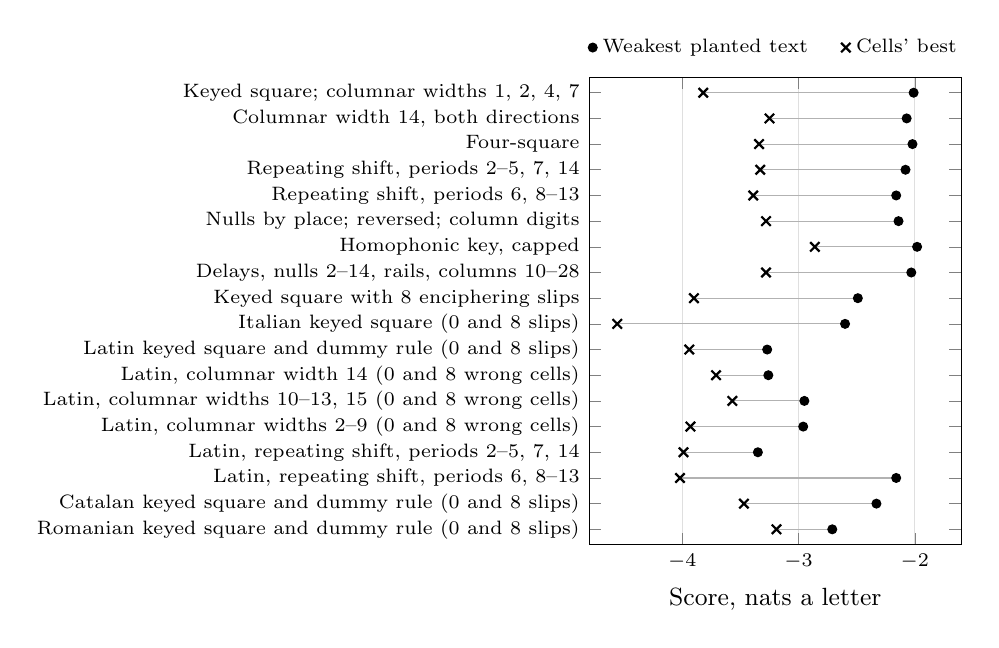
\begin{tikzpicture}
\begin{axis}[width=0.52\linewidth, height=0.62\linewidth, xmin=-4.8, xmax=-1.6,
  ymin=0.4, ymax=18.6, ytick={1,...,18}, yticklabels={{Keyed square; columnar widths 1, 2, 4, 7},{Columnar width 14, both directions},{Four-square},{Repeating shift, periods 2\textendash{}5, 7, 14},{Repeating shift, periods 6, 8\textendash{}13},{Nulls by place; reversed; column digits},{Homophonic key, capped},{Delays, nulls 2\textendash{}14, rails, columns 10\textendash{}28},{Keyed square with 8 enciphering slips},{Italian keyed square (0 and 8 slips)},{Latin keyed square and dummy rule (0 and 8 slips)},{Latin, columnar width 14 (0 and 8 wrong cells)},{Latin, columnar widths 10\textendash{}13, 15 (0 and 8 wrong cells)},{Latin, columnar widths 2\textendash{}9 (0 and 8 wrong cells)},{Latin, repeating shift, periods 2\textendash{}5, 7, 14},{Latin, repeating shift, periods 6, 8\textendash{}13},{Catalan keyed square and dummy rule (0 and 8 slips)},{Romanian keyed square and dummy rule (0 and 8 slips)}},
  y dir=reverse, yticklabel style={font=\scriptsize, align=right}, xticklabel style={font=\scriptsize},
  xlabel={Score, nats a letter}, xlabel style={font=\small}, xmajorgrids, grid style={gray!25},
  legend style={font=\scriptsize, at={(0.5,1.02)}, anchor=south, legend columns=2, draw=none,
  /tikz/every even column/.append style={column sep=1em}}, legend cell align=left]
\addplot[gray!60, forget plot] coordinates {(-3.82,1) (-2.01,1)};
\addplot[gray!60, forget plot] coordinates {(-3.25,2) (-2.07,2)};
\addplot[gray!60, forget plot] coordinates {(-3.34,3) (-2.02,3)};
\addplot[gray!60, forget plot] coordinates {(-3.33,4) (-2.08,4)};
\addplot[gray!60, forget plot] coordinates {(-3.39,5) (-2.16,5)};
\addplot[gray!60, forget plot] coordinates {(-3.28,6) (-2.14,6)};
\addplot[gray!60, forget plot] coordinates {(-2.86,7) (-1.98,7)};
\addplot[gray!60, forget plot] coordinates {(-3.28,8) (-2.03,8)};
\addplot[gray!60, forget plot] coordinates {(-3.90,9) (-2.49,9)};
\addplot[gray!60, forget plot] coordinates {(-4.56,10) (-2.60,10)};
\addplot[gray!60, forget plot] coordinates {(-3.94,11) (-3.27,11)};
\addplot[gray!60, forget plot] coordinates {(-3.71,12) (-3.26,12)};
\addplot[gray!60, forget plot] coordinates {(-3.57,13) (-2.95,13)};
\addplot[gray!60, forget plot] coordinates {(-3.93,14) (-2.96,14)};
\addplot[gray!60, forget plot] coordinates {(-3.99,15) (-3.35,15)};
\addplot[gray!60, forget plot] coordinates {(-4.02,16) (-2.16,16)};
\addplot[gray!60, forget plot] coordinates {(-3.47,17) (-2.33,17)};
\addplot[gray!60, forget plot] coordinates {(-3.19,18) (-2.71,18)};
\addplot[only marks, mark=*, mark size=1.6pt, black] coordinates {(-2.01,1) (-2.07,2) (-2.02,3) (-2.08,4) (-2.16,5) (-2.14,6) (-1.98,7) (-2.03,8) (-2.49,9) (-2.60,10) (-3.27,11) (-3.26,12) (-2.95,13) (-2.96,14) (-3.35,15) (-2.16,16) (-2.33,17) (-2.71,18)};
\addlegendentry{Weakest planted text}
\addplot[only marks, mark=x, mark size=2.4pt, thick, black] coordinates {(-3.82,1) (-3.25,2) (-3.34,3) (-3.33,4) (-3.39,5) (-3.28,6) (-2.86,7) (-3.28,8) (-3.90,9) (-4.56,10) (-3.94,11) (-3.71,12) (-3.57,13) (-3.93,14) (-3.99,15) (-4.02,16) (-3.47,17) (-3.19,18)};
\addlegendentry{Cells' best}
\end{axis}
\end{tikzpicture}

\caption{The two scores of each row of Table~\ref{tab:power}, in nats a letter under that row's language model; higher is more like the language. The dot is the row's weakest planted score, as the table defines it, and the cross the cells' best. In every row the cross lies to the left of the dot; the gap is under one nat a letter in \gapUnderOne{} rows, five of them Latin, with the Romanian row and the capped homophonic key. Rows naming no language use the English model. Scores under different models are not comparable across rows.}
\label{fig:power}
\end{figure}

\paragraph{Plain square and complete columnar transposition.} Annealing the column order and the letter key together recovers \subRecovered{} of \subPlanted{} planted texts at widths 1, 2, 4 and 7, where the cells score \subCellsLow{} to \subCellsHigh{} a letter. At width 14, which fits the $14 \times 14$ grid, a compiled kernel with \widthFourteenRestarts{} restarts of \widthFourteenSteps{} steps recovers \widthFourteenRecovered{} of \widthFourteenPlanted{} planted texts in both directions, \widthFourteenWithErrors{} of them with \widthFourteenErrors{} wrong cells; the cells and the regrouping score \widthFourteenCellsLow{} to \widthFourteenCellsHigh{}, with \widthFourteenShufflesLow{} to \widthFourteenShufflesHigh{} of \widthFourteenShuffles{} shuffles as high. An earlier pure-Python search had recovered none of three planted texts at this width.

\paragraph{Every order at small widths.} For columnar transposition in either direction with a short last row, and for periodic transposition, every order at widths 2 to 9 was scored by the mutual information of successive symbols, which no letter key can change, so the method applies to any language, but its power was shown only for English and German. In each of the \exhaustiveCases{} width and family cases, both planted texts beat the best order of a shuffle of their own symbols by more than the cells and the regrouping beat the best of three shuffles of theirs. Over all cases the planted margins are at least \exhaustivePlantedSmallest{} nats of information and the cells' at most \exhaustiveCellsLargest{}, so the separation holds case by case, not across cases. In \exAboveAll{} of the \exCasesAll{} cases the cells beat all three of their shuffles, where chance gives about \exAboveChance{} (binomial $p = \exAboveP{}$); the margins in those cases are far below the planted ones. The planted texts are compared with one shuffle and the cells with three, and at width 9 the planted margins are small, so power there is weak. At width 10 the method keeps power only for the direction called done, where planted texts beat their shuffles by at least \tenDonePlantedLow{} and the cells by \tenDoneCells{}. Double transposition with every pair of orders at widths 2 to 6, both passes in the same direction, leaves the cells below planted English and German in \doubleBelow{} of \doubleCases{} cases. \keywordCount{} keywords applied as single, double and square transpositions, \keywordOrders{} orders, bring \keywordPlantsFirst{} of \keywordPlants{} planted keywords to the top; the cells' best, \keywordCells{}, is under a shuffled copy's \keywordNullHigh{}.

\paragraph{Four-square.} With ten restarts of \fsSteps{} steps the search recovers \fsRecovered{} of \fsPlanted{} planted texts. The cells score at best \fsCellsBest{} and the regrouping \fsRegroupedBest{}, with at least \fsShufflesMin{} of \fsShuffles{} shuffles as high in every case.

\paragraph{A repeating shift on a keyed square.} The square and the shifts are annealed together, \addRestarts{} restarts of \addSteps{} steps, at periods 2, 3, 4, 5, 7 and 14 with both coordinates or the column only shifted. Planted texts are recovered \addRecovered{} of \addPlanted{} times; the miss, a column shift of period 7, ended with 84 percent of letters right. The best of \addCases{} cases on the cells and the regrouping is \addBest{}, the regrouping at period 14, where the key has the most freedom and only 3 shuffles were run; that comparison is weak, and the gap of more than one nat a letter to planted English is the result. The periods 6 and 8 to 13 were searched in a second pass with the same kernel and settings: \sgEnRecovered{} of \sgEnPlanted{} planted texts are recovered, the cells' best of \sgEnCases{} cases is \sgEnBest{}, and in \sgEnAbove{} cases the cells beat all three of their shuffles, where chance gives about \sgEnChance{}.

\paragraph{A second seed.} Seven searches were run again with a new seed: four-square and the repeating shift at every period from 2 to 14 under the English model, and the Latin searches at width 14, at widths 10 to 15, under four-square with a capped homophonic key alongside, and under the repeating shift. The other rows of Table~\ref{tab:power} have one seed. Every planted text, key, shuffle and start was drawn afresh, with the same programs, budgets and thresholds. Table~\ref{tab:reseed} gives both runs of each. In all \rsRows{} rows and under both seeds the cells score below the weakest recovered planted text, by \rsGapLow{} nats a letter at least, and recovery and the shuffle tallies are close to the first run. The smallest English gap at the second seed is \rsEnglishLow{}, for the shift at periods 6 and 8 to 13, because a weaker planted window was drawn (found at \rsEnglishLowFound{}); the cells' best there is \rsEnglishLowCells{}, against \rsEnglishLowFirstCells{} at the first seed. Latin four-square recovers \rsLaFsRecovered{} of \rsLaFsPlanted{} planted texts at the second seed, so with three planted texts that closure stays weak.

\begin{table}[t]
\centering
\caption{The searches run under two seeds. ``Found'' counts planted texts recovered with at least 90 percent of letters (or clean cells) right. ``Weakest'' is the found score per letter of the weakest recovered planted text, which differs from Table~\ref{tab:power}'s true-key score; ``Gap'' is it minus the cells' best, over the printed cells and the regrouping where the search ran it. ``As high'' counts shuffle searches reaching the cells' scores, over every case of the search. Rows naming no language use the English model.}
\label{tab:reseed}
\small
% Written by ../code/make_numbers.py. Do not edit by hand.
\begin{tabular}{@{}p{0.38\linewidth}lccccc@{}}
\toprule
Search & Seed & Found & Weakest & Cells' best & Gap & As high \\
\midrule
Four-square & first & 4/6 & \ensuremath{-1.96} & \ensuremath{-3.34} & \ensuremath{1.38} & 58/80 \\
 & second & 6/6 & \ensuremath{-1.99} & \ensuremath{-3.37} & \ensuremath{1.38} & 36/80 \\
\addlinespace[2pt]
Repeating shift, periods 2--5, 7, 14 & first & 11/12 & \ensuremath{-2.08} & \ensuremath{-3.33} & \ensuremath{1.25} & 34/72 \\
 & second & 11/12 & \ensuremath{-2.46} & \ensuremath{-3.41} & \ensuremath{0.94} & 37/72 \\
\addlinespace[2pt]
Repeating shift, periods 6, 8--13 & first & 26/28 & \ensuremath{-2.16} & \ensuremath{-3.39} & \ensuremath{1.23} & 42/87 \\
 & second & 25/28 & \ensuremath{-2.62} & \ensuremath{-3.37} & \ensuremath{0.75} & 35/87 \\
\addlinespace[2pt]
Latin, repeating shift, periods 6, 8--13 & first & 25/28 & \ensuremath{-2.78} & \ensuremath{-4.02} & \ensuremath{1.24} & 45/87 \\
 & second & 23/28 & \ensuremath{-2.75} & \ensuremath{-4.01} & \ensuremath{1.26} & 40/87 \\
\addlinespace[2pt]
Latin, columnar width 14 & first & 8/8 & \ensuremath{-3.26} & \ensuremath{-3.71} & \ensuremath{0.45} & 16/40 \\
 & second & 8/8 & \ensuremath{-3.22} & \ensuremath{-3.73} & \ensuremath{0.51} & 19/40 \\
\addlinespace[2pt]
Latin, columnar widths 10--13, 15 & first & 39/40 & \ensuremath{-2.95} & \ensuremath{-3.57} & \ensuremath{0.63} & 117/200 \\
 & second & 38/40 & \ensuremath{-2.85} & \ensuremath{-3.60} & \ensuremath{0.75} & 114/200 \\
\addlinespace[2pt]
Latin, four-square & first & 3/3 & \ensuremath{-3.27} & \ensuremath{-3.94} & \ensuremath{0.67} & 10/16 \\
 & second & 2/3 & \ensuremath{-2.45} & \ensuremath{-3.96} & \ensuremath{1.51} & 13/16 \\
\addlinespace[2pt]
Latin, capped homophonic key & first & 2/3 & \ensuremath{-1.77} & \ensuremath{-2.74} & \ensuremath{0.97} & 11/16 \\
 & second & 2/3 & \ensuremath{-1.85} & \ensuremath{-2.74} & \ensuremath{0.89} & 12/16 \\
\addlinespace[2pt]
Latin, repeating shift, periods 2--5, 7, 14 & first & 15/18 & \ensuremath{-2.73} & \ensuremath{-3.99} & \ensuremath{1.26} & 66/111 \\
 & second & 16/18 & \ensuremath{-3.07} & \ensuremath{-4.04} & \ensuremath{0.97} & 57/111 \\
\bottomrule
\end{tabular}

\end{table}

\paragraph{The book's dummies, and other short attacks.} The book allows a dummy at every third, fourth or fifth letter \cite{wikipedia2026}. Dropping every phase of those periods and of period 14 (one grid column), and reading the cells backwards, the keyed-square search recovers \quickRecovered{} of \quickPlanted{} planted texts. The cells' best over \quickVariants{} variants is \quickBest{}, a little above all \quickShuffles{} shuffles' best variants (\quickShuffleBestLow{} to \quickShuffleBestHigh{}). That edge does not survive the wider family below.

\paragraph{A homophonic key, and a trap.} Under the default model a run of one repeated letter scores above English: in a development run recorded in the development repository, the cells with every symbol sent to O scored about $-1.3$ a letter. An unconstrained many-to-one key therefore collapses onto one letter, for the cells and for their shuffles alike. Refusing any key that gives one letter more than \homCap{} places, the most the commonest letter takes in any 196-letter window of the held-out texts, the search recovers \homRecovered{} of \homPlanted{} planted homophonic texts. The cells score \homCells{}, with \homCellsAsHigh{} of \homShuffles{} shuffles as high, and the regrouping \homRegrouped{}, with \homRegroupedAsHigh{}. We record the trap because a homophonic solver without such a limit can return fluent-looking runs of frequent letters on any input.

\paragraph{Old leads.} Earlier probes, scored with an 8,689-letter model and without planted texts, left faint leads, notably a delay of 79 places between the row and the column digits that only 3 of 200 shuffles matched. \dirTransforms{} transforms were solved as keyed squares: every delay from 1 to 195, every phase of nulls at periods 2 to 14, rail fences of 2 to 14 rails and rows of 10 to 28 read down, each undone and done. Planted texts are recovered \dirRecovered{} of \dirPlanted{}. The cells' best over all transforms is \dirBest{}, and \dirAsHigh{} of \dirShuffles{} shuffles reach a best at least as high; within each of the four families 7 or 8 of 8 do. The largest single excess over a transform's own shuffles is \dirTopTransform{}, $z = \dirTopZ{}$ among \dirTransforms{} comparisons with 8 shuffles each, what the largest of so many noisy comparisons looks like.

\section{Enciphering errors and other languages}\label{sec:errors}

\paragraph{Errors.} The book's worked example has about four faults in 92 letters: 89 pairs for 92 letters, and AREA written as ARYA \cite{wikipedia2026}. At that rate the challenge might carry about eight. Most of those faults are omissions, which Proposition~\ref{prop:errors} does not count directly, but a 196-letter window of the intended passage differs from the surviving text by at most $d + k$ substitutions when $d$ letters were dropped or added and $k$ changed, so the substitution minimum over windows is still a lower bound. Under a one-to-one key, Proposition~\ref{prop:errors} answers the best case: no window of the held-out texts reaches the cells' counts with fewer than \errBestFewest{} chosen errors, and the closest window of the training prose needs \corpusClosestDistance{}. Random errors do worse. A digit slip, a wrong row or column digit, moves a letter to one of the eight cells sharing its row or column; with 4 to 48 slips or free errors, \errRandomDraws{} draws in all, no draw reaches the cells, and at least \errRandomFewest{} further errors are always needed. The search is not blinded by such errors either: planted English with 8 slips is found at \errEightLow{} a letter or better with at least \errEightRight{} percent of letters right, against the cells' \errCells{} under the same search, and planted English falls to the cells' level only at \errLevel{} errors, where \errLevelRight{} percent of its letters are right.

\paragraph{A screen of languages.} Proposition~\ref{prop:errors} needs no language model, so it can screen languages. Universal Dependencies lists \allListed{} languages with at least 5,000 tokens; for each, its largest treebank of at most 1.5 million tokens was taken. Latin-alphabet text has its accents removed, a few letters spelled out and J folded into I; Cyrillic, Greek, Armenian, Georgian and Coptic text is romanized letter by letter. \allSkippedScript{} languages written in scripts without separate vowel letters, or with signs for syllables or words, are left out, because a romanization would invent the letters being counted, \allSkippedEmpty{} treebanks carry no sentence text, and \allSkippedShort{} have too little (at most \allSkippedShortMost{} letters) for the window count, which leaves \allLanguages{}. Table~\ref{tab:screen} gives the twelve closest, and Figure~\ref{fig:screen} the median of every language. Latin stands out on the two measures that describe a language rather than one window: its median is \allLatinMedian{} against at least \allOthersMedianLow{} for every other language, and \allLatinRate{} windows per million need 8 or fewer errors, against \allSecondRate{} for the next, \allSecondRateName{}, from a corpus of only \allSecondRateLetters{} letters, and at most \allBigRateHigh{} for any other corpus of a million letters or more. Only its closest window is matched, by Estonian (\allEstonianFewest{} errors, median \allEstonianMedian{}). Russian, d'Agapeyeff's nationality until his naturalisation in 1947 \cite{gazette1947}, needs at least \ruFewest{} errors under each of four transliterations on three treebanks (\ruWithin{} windows within 8), and Esperanto, which Marland tested and set aside \cite{marland2026}, \eoFewest{} over \eoLetters{} letters of ten books. Latin was then counted at length: every window, one letter apart, of \libLetters{} letters from \libSources{} sources (treebanks and Project Gutenberg books) and of \llLetters{} letters from \llPages{} pages of The Latin Library. The closest needs \llFewest{} errors, \llWithinFour{} windows need 4 or fewer, and none comes within 2. So under a one-to-one key no Latin text in these \latinLettersAll{} million letters is a clean source; a Latin message would need a few enciphering errors, about the number the book's own example has. A count fit is a reason to search, not a reading.

\begin{table}[t]
\centering
\caption{The twelve treebanks closest to the cells' letter counts, of \allLanguages{} screened. ``Fewest'' and ``Median'' are the fewest errors (Proposition~\ref{prop:errors}) at the closest and at the median window of 196 letters; ``Within 8 per million'' is the rate of windows needing 8 or fewer. Windows are taken every few letters, at most 250,000 a treebank.}
\label{tab:screen}
\small
% Written by ../code/make_numbers.py. Do not edit by hand.
\begin{tabular}{@{}lrrrr@{}}
\toprule
Treebank & Letters & Fewest & Median & Within 8 per million \\
\midrule
Latin (ITTB) & 2{,}204{,}065 & 4 & 22 & 1{,}201 \\
Estonian (EDT) & 2{,}323{,}315 & 4 & 28 & 112 \\
Catalan (AnCora) & 2{,}171{,}416 & 5 & 28 & 33 \\
Old Occitan (CorAG) & 193{,}075 & 5 & 32 & 218 \\
Armenian (ArmTDP), romanized & 568{,}726 & 6 & 27 & 69 \\
Spanish (AnCora) & 2{,}334{,}985 & 6 & 27 & 21 \\
Buryat (BDT), romanized & 58{,}624 & 6 & 30 & 394 \\
Icelandic (IcePaHC) & 3{,}954{,}021 & 7 & 25 & 69 \\
Western Armenian (ArmTDP), romanized & 628{,}140 & 7 & 27 & 91 \\
Old East Slavic (TOROT), romanized & 1{,}135{,}032 & 7 & 32 & 22 \\
Welsh (CCG) & 208{,}261 & 8 & 26 & 19 \\
Manx (Cadhan) & 64{,}480 & 8 & 29 & 47 \\
\bottomrule
\end{tabular}

\end{table}

\begin{figure}[t]
\centering
% Written by ../code/make_numbers.py. Do not edit by hand.
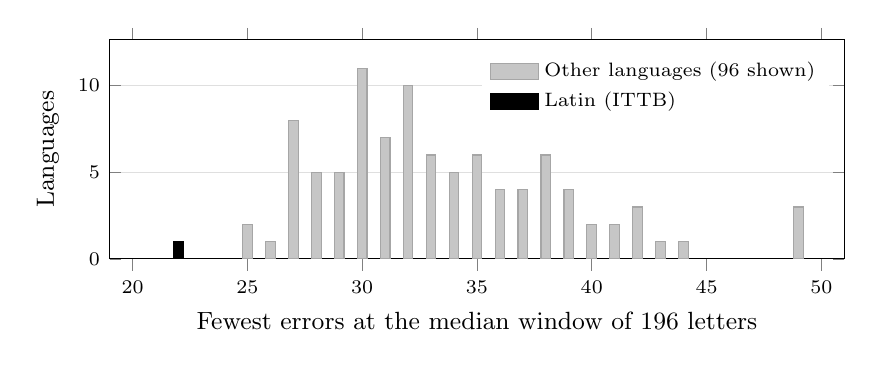
\begin{tikzpicture}
\begin{axis}[width=0.9\linewidth, height=0.36\linewidth, ybar=0pt, bar width=3.5pt, bar shift=0pt,
  xmin=19, xmax=51, ymin=0, enlarge y limits={upper, value=0.15},
  xlabel={Fewest errors at the median window of 196 letters}, ylabel={Languages},
  label style={font=\small}, ticklabel style={font=\scriptsize}, ymajorgrids, grid style={gray!25},
  legend style={font=\scriptsize, draw=none, at={(0.98,0.95)}, anchor=north east}, legend cell align=left, area legend]
\addplot[fill=gray!45, draw=gray!70] coordinates {(25,2) (26,1) (27,8) (28,5) (29,5) (30,11) (31,7) (32,10) (33,6) (34,5) (35,6) (36,4) (37,4) (38,6) (39,4) (40,2) (41,2) (42,3) (43,1) (44,1) (49,3)};
\addlegendentry{Other languages (96 shown)}
\addplot[fill=black, draw=black] coordinates {(22,1)};
\addlegendentry{Latin (ITTB)}
\end{axis}
\end{tikzpicture}

\caption{The fewest errors (Proposition~\ref{prop:errors}) at the median window of 196 letters, for each of the \allLanguages{} languages screened. Latin alone falls below 25. One language lies off the scale: \screenOutliers{}.}
\label{fig:screen}
\end{figure}

\paragraph{Italian and Latin.} An earlier pass that let each of seven languages choose a merged pair of letters had preferred Italian. With Manzoni's \emph{I promessi sposi} of 1827, \itLetters{} letters, the closest of \itWindows{} windows needs \itFewest{} errors and the median \itMedian{}. Under a quadgram model fit on its first 30 chapters, planted Italian from the remaining chapters is recovered \itRecovered{} of 4 times, and \itErrRecovered{} of 4 with 8 slips; the cells score \itCells{}, with \itAsHigh{} of 8 shuffles as high. For Latin a model was fit on \laTrainLetters{} letters of the Index Thomisticus. Planted Latin from its held-out tail and from classical Latin, which the model never saw and scores as low as \laClassicalLow{}, is recovered \laRecovered{} of 6 times, and \laErrRecovered{} of 6 with 8 slips. The cells as a keyed square score \laSquare{} (\laSquareAsHigh{} of 8 shuffles as high), and with the book's dummy rule at best \laBest{}, reached by \laBestAsHigh{} of 8 shuffles' best variants.

\paragraph{Latin under other systems.} Because a transposition keeps letter counts, the width-14 joint search of Section~\ref{sec:search} was rerun under the Latin model, starting from a Latin frequency key. It recovers \laFourteenRecovered{} of \laFourteenPlanted{} planted Latin texts in both directions, with 0 or 8 wrong cells and including classical Latin; the printed cells score \laFourteenUndone{} with the columns undone (\laFourteenUndoneHigh{} of \laFourteenShuffles{} shuffles as high) and \laFourteenDone{} done (\laFourteenDoneHigh{} of \laFourteenShuffles{}), and the regrouping is reached by at least \laFourteenRegroupedHigh{} of \laFourteenShuffles{} shuffles in each direction. The same joint search with a short last row, at widths 10, 11, 12, 13 and 15 in both directions, recovers \lwRecovered{} of \lwPlanted{} planted Latin texts, the one miss an 8-error text at width 13; the cells score \lwCellsLow{} to \lwCellsHigh{} a letter, below every recovered planted text (the weakest found at \lwWeakestFound{}), with at least \lwAsHighLow{} of 10 shuffles as high in every row. At widths 2 to 9, where the search of Section~\ref{sec:search} showed its power only on English and German, the same joint search with a quarter of the budget recovers \lsmRecovered{} of \lsmPlanted{} planted Latin texts, the weakest found at \lsmWeakestFound{}; the cells' best over both directions, the printed cells and the regrouping is \lsmBest{}, and in \lsmAbove{} of \lsmCases{} cases the cells beat all five of their shuffles, where chance gives about five. The repeating-shift count of Section~\ref{sec:counts} does not exclude Latin: Latin uses so few letters that its draws reach as few as \lmShiftFewest{} symbols, and \lmShiftReaching{} of \lmShiftDraws{} draws reaches the cells. The joint search was therefore run under the Latin model at periods 2, 3, 4, 5, 7 and 14, shifting rows, columns or both: it recovers \lsRecovered{} of \lsPlanted{} planted texts (the misses are search failures), the cells' best of \lsCases{} cases is \lsBest{}, and in \lsAbove{} cases the cells beat all three of their shuffles, where chance gives about nine. At the periods 6 and 8 to 13 the count gives Latin as few as \sgLaFewest{} symbols, though \sgLaReaching{} of \sgLaDraws{} draws reach the cells' rows as well, and the search recovers \sgLaRecovered{} of \sgLaPlanted{} planted texts, with the cells' best \sgLaBest{} and \sgLaAbove{} of \sgLaCases{} cases above all three shuffles, where chance gives about \sgLaChance{}. Four-square with standard plain squares under the Latin model recovers \lmFsRecovered{} of 3 planted texts, with \lmFsCellsHigh{} of 8 shuffles reaching the cells; a capped homophonic key recovers only \lmHomRecovered{} of 3, so that result is weaker.

\paragraph{Catalan and Romanian.} Catalan, third in Table~\ref{tab:screen}, and Romanian, fourteenth of the \allLanguages{} languages screened, were searched as Latin was, under the keyed square and the book's dummy rule, with models fit on their treebanks. Planted text is recovered 3 of 3 in each, also with 8 slips. For Catalan the cells' best, \caCells{}, is reached by \caCellsHigh{} of 8 shuffles. For Romanian it was reached by only \roCellsHigh{} of 8 at first, and the regrouping's best, \roRegroupedFirst{}, by \roRegroupedFirstHigh{} of 8. A rerun with \roWideShuffles{} shuffles gave the cells the same best, reached by \roWideHigh{} of them, and the regrouping \roRegroupedRerun{}, reached by \roWideRegroupedHigh{}; at least \roRegroupedRerunAbove{} of those shuffles exceed the first run's \roRegroupedFirst{}, so the first result was the small sample, and part of the change in the regrouping's score is search noise.

\paragraph{Latin words.} A score per letter stops separating heavily mistaken Latin from noise: planted Latin with many wrong cells is still recovered, but its found score falls toward the cells'. Words separate them. The measure is the share of letters covered by non-overlapping words of at least five letters from a vocabulary of \lwdVocab{} Latin word forms (every form seen twice in the training part of the Thomistic treebank and in PROIEL; the planted texts come from the held-out tail and from Perseus). Planted Latin under a keyed square and under width-7 columns was given 0 to \lwdErrMax{} wrong cells and decrypted with the key the search found. Clean texts are covered \lwdCleanLow{} to \lwdCleanHigh{} percent; with \lwdErrMax{} wrong cells, \lwdWorstRecovered{} of \lwdWorstPlanted{} are still recovered and coverage is \lwdWorstLow{} to \lwdWorstHigh{} percent. The printed cells, under the keyed square, the dummy rule and columnar widths 2 to 15 in both directions (\lwdSearches{} searches), reach at best \lwdCellsBest{} percent, and \lwdCellsAsHigh{} of \lwdShuffles{} shuffles searched the same way reach as much; the regrouping reaches \lwdRegroupedBest{} percent (\lwdRegroupedAsHigh{} of \lwdShuffles{} shuffles as high). \lwdAbove{} of the \lwdPlanted{} planted texts score above the cells (Figure~\ref{fig:words}). Latin with up to about one wrong cell in six, under these systems, would have shown its words.

\begin{figure}[t]
\centering
% Written by ../code/make_numbers.py. Do not edit by hand.
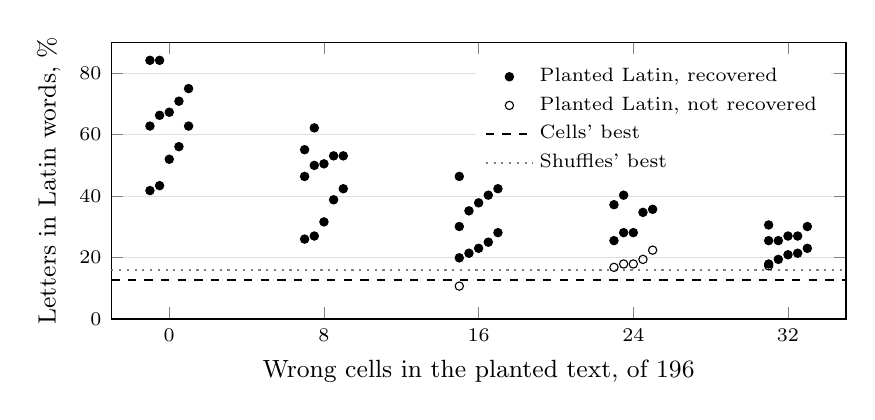
\begin{tikzpicture}
\begin{axis}[width=0.9\linewidth, height=0.42\linewidth,
  xmin=-3, xmax=35, ymin=0, ymax=90, xtick={0,8,16,24,32},
  xlabel={Wrong cells in the planted text, of 196}, ylabel={Letters in Latin words, \%},
  label style={font=\small}, ticklabel style={font=\scriptsize}, ymajorgrids, grid style={gray!25},
  legend style={font=\scriptsize, draw=none, at={(0.98,0.95)}, anchor=north east}, legend cell align=left]
\addplot[only marks, mark=*, mark size=1.5pt, black] coordinates {(-1.0,41.8) (-0.5,43.4) (0.0,52.0) (0.5,56.1) (1.0,62.8) (-1.0,62.8) (-0.5,66.3) (0.0,67.3) (0.5,70.9) (1.0,75.0) (-1.0,84.2) (-0.5,84.2) (7.0,26.0) (7.5,27.0) (8.0,31.6) (8.5,38.8) (9.0,42.4) (7.0,46.4) (7.5,50.0) (8.0,50.5) (8.5,53.1) (9.0,53.1) (7.0,55.1) (7.5,62.2) (15.0,19.9) (15.5,21.4) (16.0,23.0) (16.5,25.0) (17.0,28.1) (15.0,30.1) (15.5,35.2) (16.0,37.8) (16.5,40.3) (17.0,42.4) (15.0,46.4) (23.0,25.5) (23.5,28.1) (24.0,28.1) (24.5,34.7) (25.0,35.7) (23.0,37.2) (23.5,40.3) (31.0,17.9) (31.5,19.4) (32.0,20.9) (32.5,21.4) (33.0,23.0) (31.0,25.5) (31.5,25.5) (32.0,27.0) (32.5,27.0) (33.0,30.1) (31.0,30.6)};
\addlegendentry{Planted Latin, recovered}
\addplot[only marks, mark=o, mark size=1.5pt, black] coordinates {(15.0,10.7) (23.0,16.8) (23.5,17.9) (24.0,17.9) (24.5,19.4) (25.0,22.4) (31.0,17.3)};
\addlegendentry{Planted Latin, not recovered}
\addplot[dashed, thick, black] coordinates {(-3,12.8) (35,12.8)};
\addlegendentry{Cells' best}
\addplot[dotted, thick, gray] coordinates {(-3,16.0) (35,16.0)};
\addlegendentry{Shuffles' best}
\end{axis}
\end{tikzpicture}

\caption{Share of letters in Latin words of five letters or more, for the \lwdPlanted{} planted Latin texts by the number of wrong cells given to them, each decrypted with the key its search found; filled marks are texts recovered with at least 90 percent of clean cells right, open marks the rest, and marks are spread a little sideways so none hides another. The dashed line is the cells' best over \lwdSearches{} searches and the dotted line the best of the \lwdShuffles{} shuffles searched the same way.}
\label{fig:words}
\end{figure}

\section{Starting from no message}\label{sec:nomessage}

Van Eykelen's recipe \cite{vaneykelen2026xv} can be stated as a null hypothesis and tested. Under it the cells are their own symbols dealt onto the grid at random, the rare symbols at row ends; here the \nmFixed{} rare cells are held in place and the other cells are dealt at random. The letter counts are then fixed, and only the order can separate a message from no message. Thirty order statistics, declared before any score was read and unchanged by any one-to-one key, were used: the share of equal symbols and the mutual information of symbols at each lag from 1 to 14, the number of different neighbouring pairs and the number of repeated triples. Each statistic gets a two-sided rank p-value against 20,000 dealings, and the family-wise p-value is the share of dealings whose smallest p-value is as small as the cells'.

The cells give a family-wise p-value of \nmFamilyP{}. Their smallest single p-value, \nmSmallestP{}, is the mutual information at lag 3, the trace van Eykelen reported; it does not survive the correction for thirty statistics, and finding it again on the same cells is not independent confirmation. Table~\ref{tab:nomessage} gives the test's power: planted held-out English hidden by five message systems, each tested against dealings of its own symbols.

\begin{table}[t]
\centering
\caption{Power of the no-message test. Planted held-out English texts flagged at a family-wise p-value of 0.05 or less, out of \nmPlanted{} per system. Each planted text is tested against \nmPlantNull{} dealings of all 196 of its symbols with no places held; only the cells are tested against \nmCellNull{} dealings with \nmFixed{} places held. A random transposition of the planted text is itself a no-message dealing, the calibration case.}
\label{tab:nomessage}
\small
\begin{tabular}{@{}lc@{}}
\toprule
Message system & Flagged \\
\midrule
Keyed square (any one-to-one key) & \nmSquare{} \\
14-column transposition, done & \nmDone{} \\
Repeating coordinate shift, periods 2 to 14 & \nmShift{} \\
Turning grille, $14 \times 14$ & \nmGrille{} \\
14-column transposition, undone & \nmUndone{} \\
Random transposition (calibration) & \nmRandom{} \\
\bottomrule
\end{tabular}
\end{table}

The order of the cells is consistent with a no-message dealing, by a test that would almost always have caught a message under a keyed square or a done 14-column transposition. Its power was measured on planted English only, under the five systems of the table: it flags a repeating shift \nmShift{} of \nmPlanted{} times, and it nearly cannot see systems that scramble order thoroughly, the turning grille and the undone 14-column transposition. The second is closed by the joint searches for English and Latin. Among these five systems, then, the order leaves two explanations: no message, or a message under a system that destroys order as completely as a turning grille. The first is simpler; neither is proved, and systems outside the five were not measured.

\section{What remains open}\label{sec:open}

The width-14 transposition was searched under English and Latin models; other languages under it are open. The small-width searches of Section~\ref{sec:search} use a score no letter key can change, but their power was shown only for English and German; for Latin a joint search with shown Latin power covers the same widths. The $14 \times 14$ turning grille, the main message system among those whose order was tested in Section~\ref{sec:nomessage}, is not closed: a compiled search recovers \grilleKnown{} planted grilles with the letter key given, but \grilleJoint{} with grille and key both unknown, at most \grilleJointHolesHigh{} of 49 holes right after \grilleJointSteps{} steps, so the cells were not searched with it. Under the Latin model the grille search with the key held fixed recovers \lgExact{} of \lgPlanted{} planted grilles with the true key, \lgMid{} of \lgPlanted{} with keys \lgMidLow{} to \lgMidHigh{} percent right and \lgLow{} of \lgPlanted{} with keys \lgLowLow{} to \lgLowHigh{} percent right, while re-solving the key at every grille move recovers \lgNested{} of \lgNestedOf{} (at most \lgNestedHoles{} holes); the grille can be found only from a nearly right key, and key-only methods so far reach about 59 percent. Four-square with keyed plain squares and two-square are not excluded by the count, and a search annealing all four squares (with the move set of the two-square solver in Colossus) recovered \ksRecovered{} of \ksPlanted{} planted texts after \ksSteps{} steps, its wrong keys reaching \ksWrong{} a letter; at 196 letters it has no power, so the cells were not searched. A general table from letter pairs to cell pairs, such as a $2 \times 2$ Hill cipher over a keyed square, is not excluded by the pair count, which is ordinary for prose (\pairCellsAMany{} and \pairCellsBMany{} windows have as many different pairs as the cells). For English, columnar transposition at widths 11 to 13 and above 14 is open as a search, though the letter counts of Section~\ref{sec:counts} already exclude ordinary English under any transposition and a one-to-one key unless about \corpusClosestDistance{} errors were chosen to fit them (Section~\ref{sec:errors}); for Latin it is closed at widths 2 to 15 and open above. Double transposition above width 6 is open in every language, for which divide-and-conquer methods exist \cite{lasry2014}; under the Latin model a joint search of both orders and the key recovers \ldSmall{} of \ldSmallOf{} planted texts at 4 by 5 and 5 by 7, but \ldSix{} of \ldSixOf{} at 6 by 8 and \ldLarge{} at 7 by 9 and 9 by 11. Finally, a construction with no message, such as van Eykelen's tally-and-deal recipe \cite{vaneykelen2026xv}, is consistent with every count and score reported here, and passes the order test of Section~\ref{sec:nomessage}.

\section{Conclusion}\label{sec:conclusion}

No reading is found and none is claimed. Two statements are results. First, under a one-to-one key, with or without a transposition, the cells are not ordinary English unless about \corpusClosestDistance{} errors were chosen to fit the letter counts. The closest of \corpusWindows{} windows of English prose needs \corpusClosestDistance{} errors, about as many faults as the book's worked example suggests; random slips at that rate leave every held-out text at least \errRandomFewest{} errors short (Section~\ref{sec:errors}). Every English search with a one-to-one key and shown power leaves the cells below the weakest planted text of Table~\ref{tab:power} by at least \gapEnglishLow{} nats a letter, and by \rsEnglishLow{} at the least under a second seed (Table~\ref{tab:reseed}); the capped homophonic key, which is not one-to-one, closes by only \gapHomTab{}. Second, under the same keys, Latin is the one language the count screen singles out: its median window needs \allLatinMedian{} errors, against at least \allOthersMedianLow{} for every other language screened, and \allLatinRate{} of its windows per million need 8 or fewer. Yet no Latin text in \latinLettersAll{} million letters is a clean source, and every Latin search with shown power found nothing (Section~\ref{sec:errors}).

On this evidence our reading is that the challenge most likely carries no message. That is an interpretation, not a result, and it rests on two things: no search with shown power found a message, and a construction with no message reproduces every count and score reported here and passes the order test of Section~\ref{sec:nomessage}. Consistency is not proof: the order test is nearly blind to a turning grille, and the families of Section~\ref{sec:open} remain open. If the cells do hold a message in a natural language under a one-to-one key, the counts point to Latin, not English; the screen's Latin is the medieval Latin of the Index Thomisticus. The languages that descend from Latin are not singled out: Spanish, Catalan and Old Occitan have medians of 27 to 32 (Table~\ref{tab:screen}), against \corpusMedianErrors{} for English prose. The challenge's omission from the editions of 1952 onward \cite{numberworld2015}, and the report that its author later forgot his method \cite{wikipedia2026}, for which Snider notes that no primary source has been located \cite{snider2026}, fit this reading, but they fit a lost key equally well and are given no weight here.

\section{Limitations}\label{sec:limits}

The 1939 book is known here from the transcription on the English Wikipedia page \cite{wikipedia2026}: the digits, the worked exercise and its square, and the dummy rule; page numbers for the book differ between sources. The block agrees digit for digit with two other public transcriptions \cite{ashley2026,snider2026}, which may share its source. Known from its bibliographic record: Barker \cite{barker1978}. Known from search summaries: Shulman \cite{shulman1952}, Schmeh \cite{schmeh2026mtc3} and the two blog series \cite{pleasedecipher2010,numberworld2015}. Known from their Zenodo records as read on 5 October 2026: the three published readings \cite{uygun2026,caillahua2026,leggett2025}. The counts in Section~\ref{sec:counts} are taken over windows of particular corpora, and English prose of other kinds, such as telegraphese with abbreviations, may vary more. The counts for the repeating shift and for four-square with keyed plain squares assume a key drawn independently of the text; chosen plain squares defeat the four-square count. The searches measure power on held-out prose of the same length; a plaintext very unlike that prose could be missed. The decision that a family is closed rests on two comparisons, planted text against the cells and the cells against their shuffles; the thresholds (90 percent of letters, a gap of about one nat a letter) are judgments and were not formally registered in advance, and several controls use few shuffles. \gapUnderOne{} of the \gapRows{} families of Table~\ref{tab:power} close with a gap under one nat a letter, \gapLatinUnder{} of the \gapLatinRows{} Latin rows (\gapLatinLow{} to \gapLatinUnderHigh{}), Romanian (\gapRomanianTab{}) and the capped homophonic key (\gapHomTab{}); those closures are weaker than the others. Under a second seed the English shift at periods 6 and 8 to 13 closes by only \rsEnglishLow{} (Table~\ref{tab:reseed}). The language screen uses mixed-genre treebank sentences, one folding convention for each script, and a letter-by-letter romanization for the non-Latin alphabets; scripts without vowel letters were not screened. Our survey of prior work is bounded by the sources listed, several of which were read through search summaries; absence from it does not show that a result is new.

\section{Reproducibility}\label{sec:repro}

Every probe is a module of the development repository, \url{https://github.com/ChaseHendrick/Undeciphered-Texts}, under \texttt{engine/}, with a test under \texttt{tests/} and a dated note under \texttt{docs/logs/}. Each writes its result once to \texttt{engine/data/swarm\_cache/}, and later calls read that file; deleting a file reruns its search, which takes from seconds to about thirty minutes on four cores and needs a C compiler. Probes that use outside text (Manzoni, the treebanks, Project Gutenberg books, The Latin Library) fetch it into an ignored folder and store only counts and scores; the romanization of non-Latin alphabets uses the \texttt{unidecode} package. The numbers and tables of this manuscript are written by \texttt{code/make\_numbers.py} from those files, whose SHA-256 hashes head \texttt{paper/numbers.tex}; it refuses any file that claims a reading, and with \texttt{--check} it fails if any number printed here no longer matches its file.

{\raggedright\noindent\textbf{Data availability.} The manuscript, \texttt{code/make\_numbers.py}, the frozen result of every probe cited here (\texttt{data/swarm\_cache/}), the held-out texts whose letters are counted (\texttt{data/texts/}) and the cells (\texttt{data/cells.json}) are in the companion repository, \url{https://github.com/ChaseHendrick/dagapeyeff}, whose releases are archived as preprints on Zenodo with the manuscript, every version at \url{https://doi.org/10.5281/zenodo.23241303}. Each release names the commit of the development repository it was published from.\par}

\noindent\textbf{Funding.} This research received no external funding.

\noindent\textbf{Use of AI.} This work was prepared with AI assistance. The author takes full responsibility for its content.

{\raggedright\noindent\textbf{Rights.} Copyright (c) 2026 Chase Hendrick. The manuscript is all rights reserved. Code and data are licensed under Apache-2.0, subject to component notices.\par}

\bibliographystyle{plain}
\bibliography{refs}

\end{document}
